% Copyright 2004 by Till Tantau <tantau@users.sourceforge.net>.
%
% In principle, this file can be redistributed and/or modified under
% the terms of the GNU Public License, version 2.
\documentclass{beamer}

% themes: http://deic.uab.es/~iblanes/beamer_gallery/index_by_theme.html
%\usetheme{Goettingen}
\usetheme{Copenhagen}

\title{Product Recommendation by Rating-based Collaborative Filtering using Apache Spark}

% \subtitle{Optional Subtitle}

\author{Songxiao Zhang \and Alan Yang \and Suzanne McIntosh}

\institute[New York University] 
{
  Courant Institute of Mathematical Sciences,\\
  New York University \\
  \bigbreak
  \{sz1451, asy233, sm4971\}@nyu.edu
}

\date{May, 2016}

%\pgfdeclareimage[height=0.7cm]{university-logo}{image/cims_banner}{my
%\logo{\pgfuseimage{university-logo}}


\AtBeginSubsection[]
{
  \begin{frame}<beamer>{Outline}
    \tableofcontents[currentsection,currentsubsection]
  \end{frame}
}

\begin{document}

\begin{frame}
  \titlepage
\end{frame}


%%%%%%%%%%%%%%%%%%%%%%%%%%%%%%%%%%%%%%%%%%%%%%%%%%%%%%%%%%%%%%%%%%%%%%%%%%%%%%%%%%%%
%%%%%%%%%%%%%%%%%%%%%%%%%%%%%%%%%%%%%%%%%%%%%%%%%%%%%%%%%%%%%%%%%%%%%%%%%%%%%%%%%%%%

\begin{frame}{Abstract}{}

  \begin{itemize}

      \item{ Explore whether we can create a solid recommendation system based on user high user ratings/reviews on certain products}
      
      \item{ Collaborative filtering - technique commonly used for recommendation systems.}
      
      \item{ Model based - develop descriptive model of user ratings with ML approaches. Use generated model for future prediction on the user's preference}
 
  \end{itemize}
  
\end{frame}

%%%%%%%%%%%%%%%%%%%%%%%%%%%%%%%%%%%%%%%%%%%%%%%%%%%%%%%%%%%%%%%%%%%%%%%%%%%%%%%%%%%%
%%%%%%%%%%%%%%%%%%%%%%%%%%%%%%%%%%%%%%%%%%%%%%%%%%%%%%%%%%%%%%%%%%%%%%%%%%%%%%%%%%%%

\begin{frame}{Motivation}{}

  \begin{itemize}

      \item{ Who are the users of this analytic?}
      \begin{itemize}
          \item {E-commerce sites that are exploring better recommendation systems}
      \end{itemize}
      \item{ Who will benefit from this analytic?}
      \begin{itemize}
          \item {E-commerce sites - sell more products and improve user experience}
          \item{Site users/buyers - get recommended with products they may be interested in, better experience}
      \end{itemize}
      
      \item{ Why is this analytic important?}
      \begin{itemize}
          \item {E-commerce sites are a big part of our community and economy now.}
          \item{Advantage of directly recommended items to make up for lack of browsing efficiency like in real store.}
      \end{itemize}
 
  \end{itemize}
  
\end{frame}

%%%%%%%%%%%%%%%%%%%%%%%%%%%%%%%%%%%%%%%%%%%%%%%%%%%%%%%%%%%%%%%%%%%%%%%%%%%%%%%%%%%%
%%%%%%%%%%%%%%%%%%%%%%%%%%%%%%%%%%%%%%%%%%%%%%%%%%%%%%%%%%%%%%%%%%%%%%%%%%%%%%%%%%%%

\begin{frame}{Goodness}
  \begin{itemize}
  \item {
    Data from reliable E-commerce sources (Amazon, Yelp)
  }
  \item {   
    Data split into training and testing and validation segments
  }
  \item {
    RMSE (Root Mean Square Error) 
  }
  \item {
    Looking and personal intuition
  }
  \end{itemize}
\end{frame}

%%%%%%%%%%%%%%%%%%%%%%%%%%%%%%%%%%%%%%%%%%%%%%%%%%%%%%%%%%%%%%%%%%%%%%%%%%%%%%%%%%%%
%%%%%%%%%%%%%%%%%%%%%%%%%%%%%%%%%%%%%%%%%%%%%%%%%%%%%%%%%%%%%%%%%%%%%%%%%%%%%%%%%%%%
\begin{frame}{Data Sources}
  \begin{enumerate}
      \item {Amazon Review Data}
      \begin{itemize}
          \item {Amazon data provided by Dr. Julian McAuley from UCSD}
          \item{Consists of: \textbf{reviewerID}, \textbf{asin} (Amazon Standard Identification Number), reviewerName, helpful, \textbf{stars}, reviewText, \textbf{overall} (rating), summary, unixReviewTime, reviewTime}
          \item {Size of Data: 6.6GB of review data, 1.2GB of metadata used}
      \end{itemize}
      \item{Yelp Review Data}
      \begin{itemize}
          \item {Yelp data taken from a Yelp Data Set Challenge: \url{https://www.yelp.com/dataset_challenge} }
          \item{Consists of: votes, \textbf{userID}, reviewID, \textbf{stars}, date, text, type, \textbf{businessID}}
          \item{Size of Data: 1.9GB of review data, and 66MB of metadata used}
      \end{itemize}
  \end{enumerate}
\end{frame}


%%%%%%%%%%%%%%%%%%%%%%%%%%%%%%%%%%%%%%%%%%%%%%%%%%%%%%%%%%%%%%%%%%%%%%%%%%%%%%%%%%%%
%%%%%%%%%%%%%%%%%%%%%%%%%%%%%%%%%%%%%%%%%%%%%%%%%%%%%%%%%%%%%%%%%%%%%%%%%%%%%%%%%%%%

\begin{frame}{Design}{}

 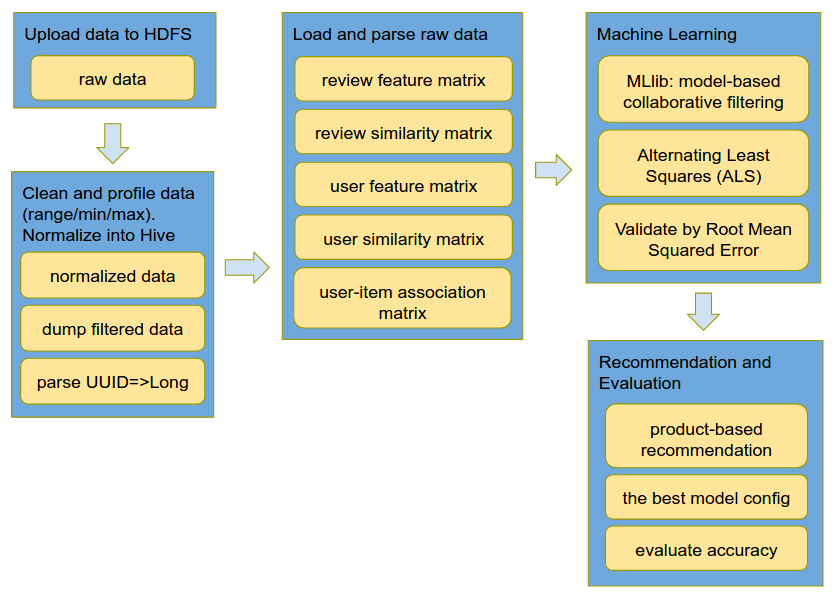
\includegraphics[width=1\textwidth]{image/design_v2}
 
  
\end{frame}

%%%%%%%%%%%%%%%%%%%%%%%%%%%%%%%%%%%%%%%%%%%%%%%%%%%%%%%%%%%%%%%%%%%%%%%%%%%%%%%%%%%%
%%%%%%%%%%%%%%%%%%%%%%%%%%%%%%%%%%%%%%%%%%%%%%%%%%%%%%%%%%%%%%%%%%%%%%%%%%%%%%%%%%%%

\begin{frame}{Design}{}

    \begin{itemize}
        \item {Platform: Hive and MLlib ran on NYU HPC Cluster - Dumbo}
     
        \item{Tools: Hive, Apache Spark, MLlib - ALS algorithm}
        
        \item{Dataset split into $60\%$ for training, $20\%$ for testing and $20\%$ for validation}
        
        \item {
            
            Low-rank matrix factorization 
            $$U[i] = \min_{w \in \mathbb{R}^d} \sum_{j \in Nbrs(i))} (r_{ij} - w^TV^T[j])^2 + \lambda \left \| w \right \|^2_2$$
            
            Root Mean Squared Error (RMSE) amplifies and severely punishes large errors comparing to Mean Absolute Error
            $$RMSE = \sqrt{\frac{1}{n} \sum_{i=1}^{n}(y_i - \hat{y_i})^2}$$
            
        }
    \end{itemize}
 
\end{frame}


%%%%%%%%%%%%%%%%%%%%%%%%%%%%%%%%%%%%%%%%%%%%%%%%%%%%%%%%%%%%%%%%%%%%%%%%%%%%%%%%%%%%
%%%%%%%%%%%%%%%%%%%%%%%%%%%%%%%%%%%%%%%%%%%%%%%%%%%%%%%%%%%%%%%%%%%%%%%%%%%%%%%%%%%%

\begin{frame}{Collaborative Filtering Recommendation Systems}{}
\begin{minipage}{0.5\textwidth}
    \begin{figure}[H]
    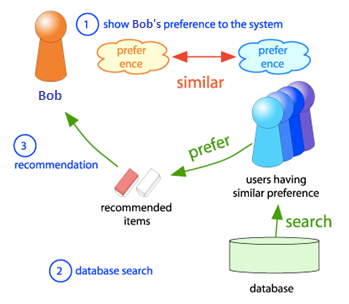
\includegraphics[width=1\textwidth]{image/cf_example_flow}
    \caption{\label{fig:CF} Collaborative Filtering}
    \end{figure}
    \end{minipage} \hfill
    \begin{minipage}{0.45\textwidth}
  \begin{enumerate}
      \item {
        First consider Bob.
      }
      \item {
        Find set N of other users who has same rating of 5 as Bob.
      }
      \item {
        Estimate Bob's ratings of other products based on ratings of users in N.
      }
      \item {
        Same idea here, based on the similar product ratings, find other products that they would both be interested in.
      }
  \end{enumerate}
  \end{minipage}

\end{frame}

%%%%%%%%%%%%%%%%%%%%%%%%%%%%%%%%%%%%%%%%%%%%%%%%%%%%%%%%%%%%%%%%%%%%%%%%%%%%%%%%%%%%
%%%%%%%%%%%%%%%%%%%%%%%%%%%%%%%%%%%%%%%%%%%%%%%%%%%%%%%%%%%%%%%%%%%%%%%%%%%%%%%%%%%%

\begin{frame}{Results - Yelp Data}{}

  \begin{itemize}
      \item {
        RMSE (validation) = 3.950921 for the model trained with rank = 8, lambda = 0.1, and numIter = 1.
        RMSE on the test set is 3.952831
      }
      \item {
        Most places in the input data is in NV and AZ.
      }
      \item {
        Results are mostly in NV and AZ as well, which helps us think that our results are semi-reliable through intuition.
      }
  \end{itemize}
  
\end{frame}

%%%%%%%%%%%%%%%%%%%%%%%%%%%%%%%%%%%%%%%%%%%%%%%%%%%%%%%%%%%%%%%%%%%%%%%%%%%%%%%%%%%%
%%%%%%%%%%%%%%%%%%%%%%%%%%%%%%%%%%%%%%%%%%%%%%%%%%%%%%%%%%%%%%%%%%%%%%%%%%%%%%%%%%%%

\begin{frame}{Results - Yelp Data}{}

    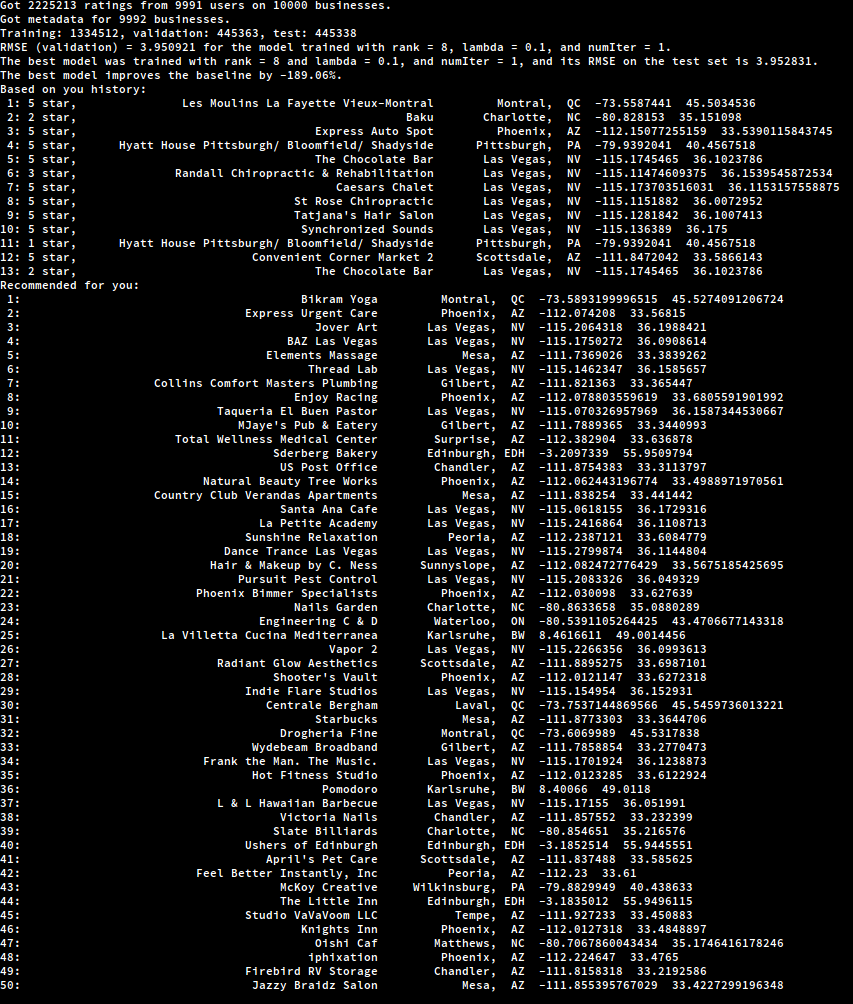
\includegraphics[width=.98\textwidth, clip=true, trim = 0cm 17cm 4cm 1cm]{image/yelp_results}
    %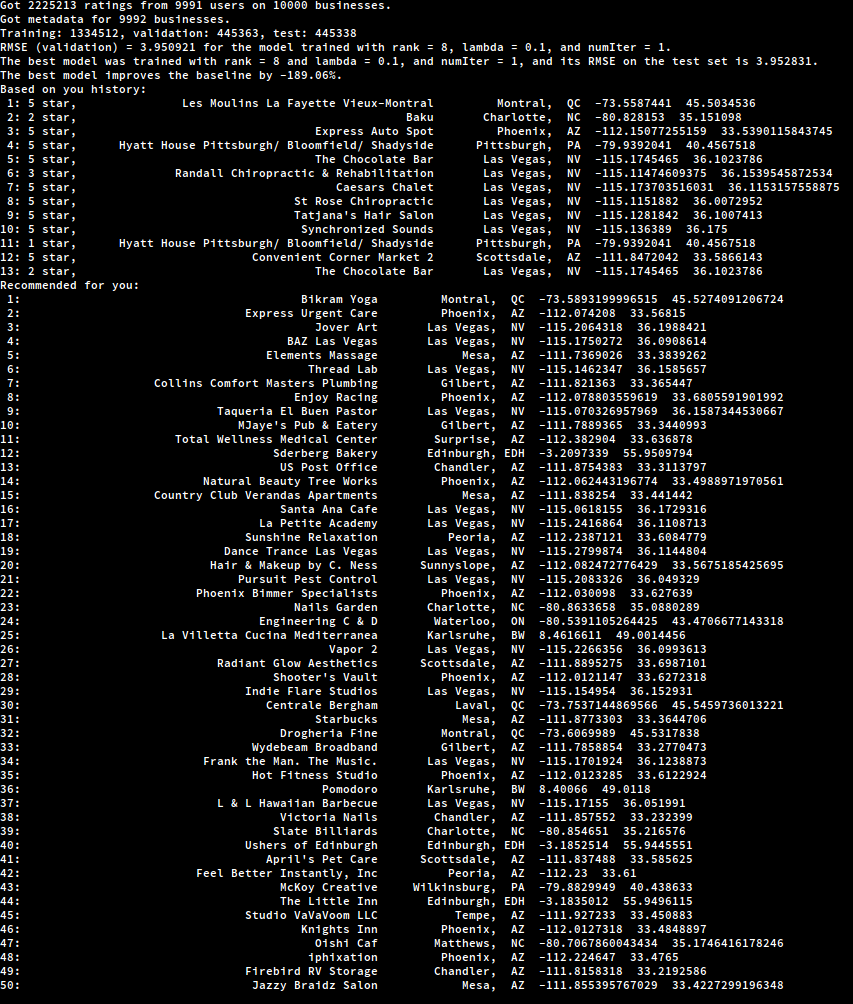
\includegraphics[width=1\textwidth]{image/yelp_results}
  
\end{frame}

%%%%%%%%%%%%%%%%%%%%%%%%%%%%%%%%%%%%%%%%%%%%%%%%%%%%%%%%%%%%%%%%%%%%%%%%%%%%%%%%%%%%
%%%%%%%%%%%%%%%%%%%%%%%%%%%%%%%%%%%%%%%%%%%%%%%%%%%%%%%%%%%%%%%%%%%%%%%%%%%%%%%%%%%%

\begin{frame}{Results - Amazon Data}{}

  \begin{itemize}
      \item {
        RMSE (validation) = 3.066711 for the model trained with rank = 8, lambda = 0.1, and numIter = 1.
        RMSE on the test set is 3.066156.
      }
      \item {
        From the user's input data we notice makeup and woman shirts among other woman products.  But this woman also seems to enjoy certain pro-shop past times, maybe hunting or shooting, because of 5 star dart rating and pro shop apron.
      }
      \item {
        Some of the results are either woman products such as beauty products and woman clothes, but in there are also some pro shop items such as fishing gear.
      }
      \item {
        It's harder to use intuition to validate Amazon results.
      }
  \end{itemize}
  
\end{frame}

%%%%%%%%%%%%%%%%%%%%%%%%%%%%%%%%%%%%%%%%%%%%%%%%%%%%%%%%%%%%%%%%%%%%%%%%%%%%%%%%%%%%
%%%%%%%%%%%%%%%%%%%%%%%%%%%%%%%%%%%%%%%%%%%%%%%%%%%%%%%%%%%%%%%%%%%%%%%%%%%%%%%%%%%%

\begin{frame}{Results - Amazon Data}{}

      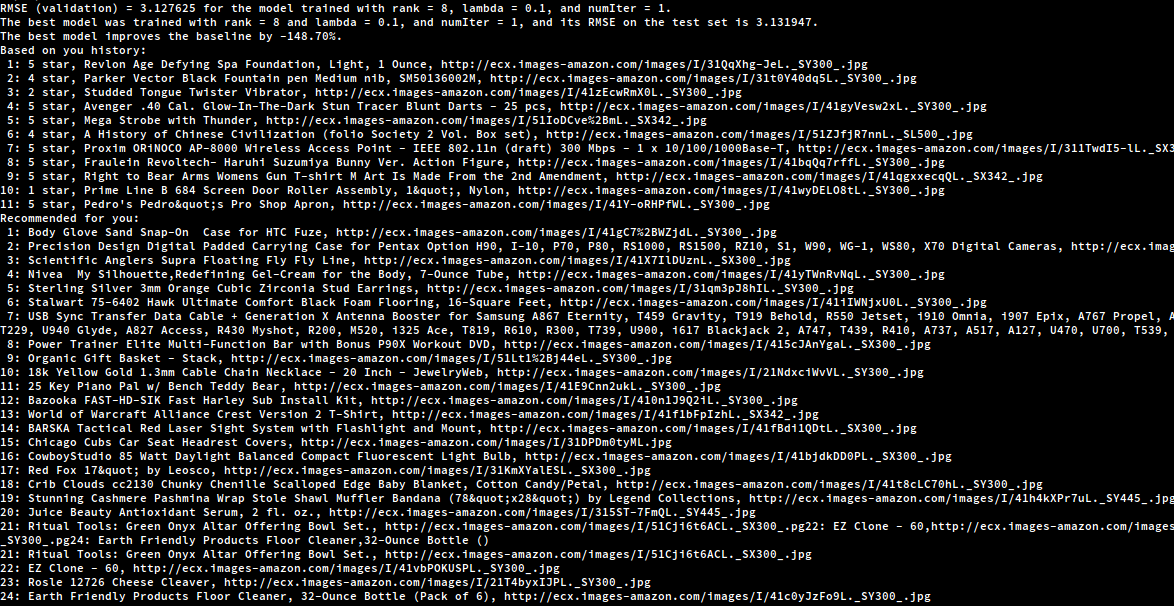
\includegraphics[width=.98\textwidth, clip=true, trim = 0cm 1cm 7cm 0cm]{image/amazon_results_crop}
  
\end{frame}



%%%%%%%%%%%%%%%%%%%%%%%%%%%%%%%%%%%%%%%%%%%%%%%%%%%%%%%%%%%%%%%%%%%%%%%%%%%%%%%%%%%%
%%%%%%%%%%%%%%%%%%%%%%%%%%%%%%%%%%%%%%%%%%%%%%%%%%%%%%%%%%%%%%%%%%%%%%%%%%%%%%%%%%%%

\begin{frame}{Obstacles}

  \begin{itemize}
      \item { MLlib's ALS algorithm training function asks for Java int variables as its mapped training data, and so our alpha-numeric ids for Yelp data do not work without some data manipulation }
      \item { java heap space out of memory for Amazon Data, This is because the available free memory on HPC is too low, and we have too much data, works if we significantly cut down our data}
  \end{itemize}
  
\end{frame}


%%%%%%%%%%%%%%%%%%%%%%%%%%%%%%%%%%%%%%%%%%%%%%%%%%%%%%%%%%%%%%%%%%%%%%%%%%%%%%%%%%%%
%%%%%%%%%%%%%%%%%%%%%%%%%%%%%%%%%%%%%%%%%%%%%%%%%%%%%%%%%%%%%%%%%%%%%%%%%%%%%%%%%%%%
% Placing a * after \section means it will not show in the
% outline or table of contents.

\begin{frame}{Summary}
  \begin{itemize}
    \item{
    We trained our models on the training set and selected the best model on the validation set based on the lowest RMSE.  The best model is then evaluated on our test set.
    }
  \item {
    We were able to get recommendations for both yelp and amazon data using CF and MLlib's ALS algorithm
    }
    \item{
    To verify if these recommended items are true or false really depends on the user himself
    }
  \end{itemize}
  
  \begin{itemize}
  \item
    Acknowledgements
    \begin{itemize}
    \item
      Professor McIntosh for the advise throughout the project
    \item
      Dr. Julian McAuley from UCSD for the Amazon review data
    \item
      Yelp Dataset Challenge board for the Yelp review data
    \item
      Wensheng Deng, Stratos Efstathiadis, and Santhosh Konda from NYU HPC
    \end{itemize}
  \end{itemize}
\end{frame}
%%%%%%%%%%%%%%%%%%%%%%%%%%%%%%%%%%%%%%%%%%%%%%%%%%%%%%%%%%%%%%%%%%%%%%%%%%%%%%%%%%%%

\appendix
\section<presentation>*{\appendixname}
\subsection<presentation>*{References}

\begin{frame}[allowframebreaks]
  \frametitle<presentation>{References}
    
  \begin{thebibliography}{10}
    
  \beamertemplateonlinebibitems
  % Start with overview books.

    \bibitem{ApacheSpark}
    Apache Spark, 
    \newblock{\url{http://spark.apache.org/}}
    
    \bibitem{YelpDataset}
    \newblock{Yelp Dataset Challenge,}
    \newblock{\url{https://www.yelp.com/dataset_challenge}}
    
    \beamertemplatearticlebibitems
    \bibitem{Image-based}
    J. McAuley, C. Targett, J. Shi, A. van den Hengel. \newblock{Image-based recommendations on styles and substitutes.}
    \newblock{SIGIR, 2015}
    
    \bibitem{substitutable}
    J. McAuley, R. Pandey, J. Leskovec. 
    \newblock{Inferring networks of substitutable and complementary products.}
    \newblock{Knowledge Discovery and Data Mining, 2015}

    \bibitem{ClusteringItems}
    M. O’Connor, J. Herlocker. 
    \newblock{Clustering Items for Collaborative Filtering.} \newblock{In: Proceedings of the ACM SIGIR Workshop on Recommender Systems, Berkley, USA, 25-26 August, 1999}
    
    \bibitem{Multi-view}
    Pradhan, L., Zhang, C., \& Chitrakar, P. (2016). \newblock{Multi-view Clustering in Collaborative Filtering Based Rating Prediction.}
    \newblock{In: 2016 IEEE Tenth International Conference on Semantic Computing (ICSC).} $doi:10.1109/icsc.2016.40$
    \beamertemplatebookbibitems
    \bibitem{Resnick}
    Resnick, P., Iacovou, N., Suchak, M., Bergstrom, P., and Riedl, J. (1994). 
    \newblock{Grouplens: An open architecture for collaborative filtering of netnews.}
    \newblock{ In: Proceedings of the ACM 1994 Conference on Computer Supported Cooperative Work, pages 175-186, New York. ACM.}
    
    \beamertemplatearticlebibitems
    \bibitem{Breese}
    Breese, J., Heckerman, D., and Kadie, C. (May, 1998).
    \newblock{An experimental comparison of collaborative filtering methods.}
    \newblock{Technical Report MSR-TR-98-12, Microsoft Research, Redmond, WA.}

  \end{thebibliography}
\end{frame}

\end{document}

